\begin{figure}[t]
 \centering
  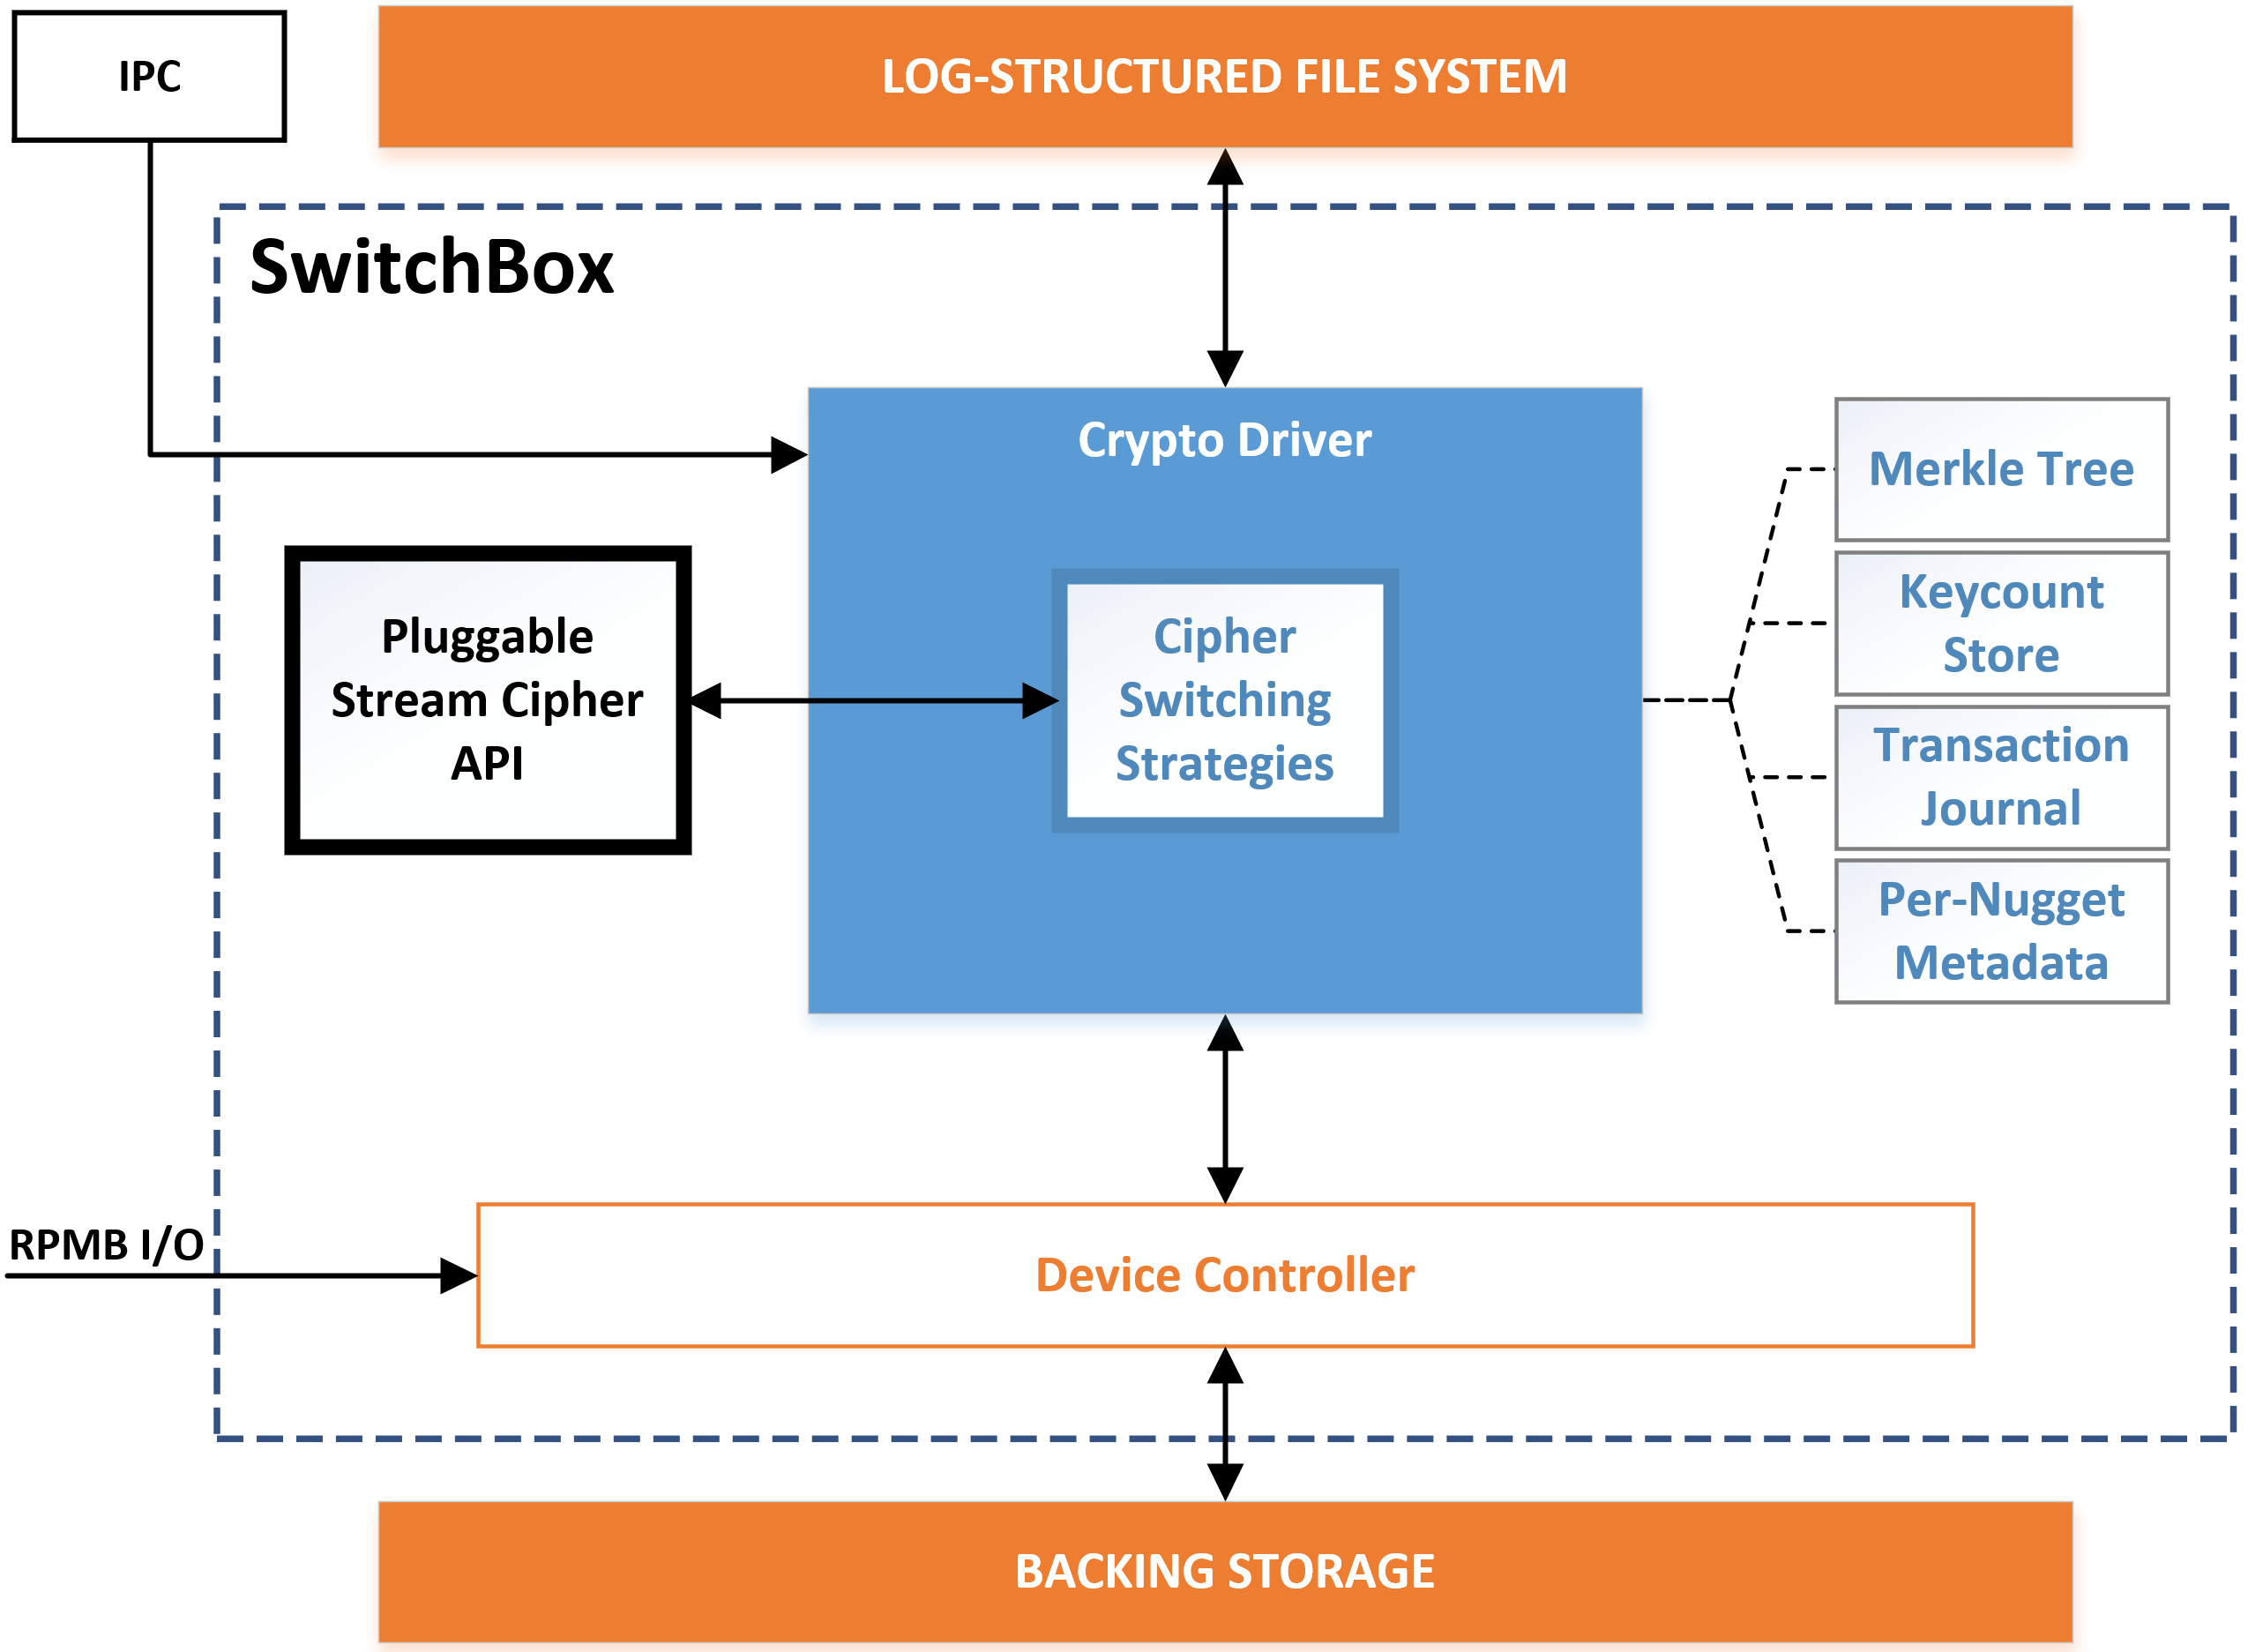
\includegraphics[width=\linewidth]{overview.png}
   \caption{Overview of the \SYSTEM{} construction.}\label{fig:overview}
\end{figure}

\section{\SYSTEM{} Design}\label{sec:design}

\TODO{Exactly how much of the original StrongBox should be explained here? Is
this too much? Too little?}

\SYSTEM{}, like StrongBox, is a translation layer positioned between the block
layer and the operating system's virtual file system~\cite{StrongBox}. There are
several places \SYSTEM{} could be implemented in the system stack: as part of an
actual kernel Log-structured File System (LFS) module like the F2FS filesystem,
as a block device or virtual block device in the manner of dm-crypt, or within a
device controller such as an SSD drive controller's FTL~\cite{StrongBox}.

\figref{overview} illustrates the \SYSTEM{} design. \SYSTEM{} manages five
metadata components: an in-memory \emph{Merkle Tree}; two drive-backed byte
arrays, \ie{the \emph{Keycount Store} and the \emph{Transaction Journal}}; a
globally persistent cryptographically secure monotonic counter; and a flexible
drive-backed per-nugget metadata store. For our monotonic counter
implementation, we used a \emph{Replay Protected Memory Block} (RPMB).

These five components are tightly integrated into the cryptographic driver,
which interacts with 1) the underlying backing store through the device
controller block I/O layer as well as 2) the overlying LFS through traditional
I/O passed through the Linux Virtual Filesystem Switch (VFS). The cryptographic
driver handles data encryption, decryption, overwrite detection, integrity
protection, and the application of cipher switching strategies.

\TODO{Should we also talk about the layout of the backing store? It's pretty
much the same as StrongBox's with an extra header}

\begin{figure}[t]
 \centering
  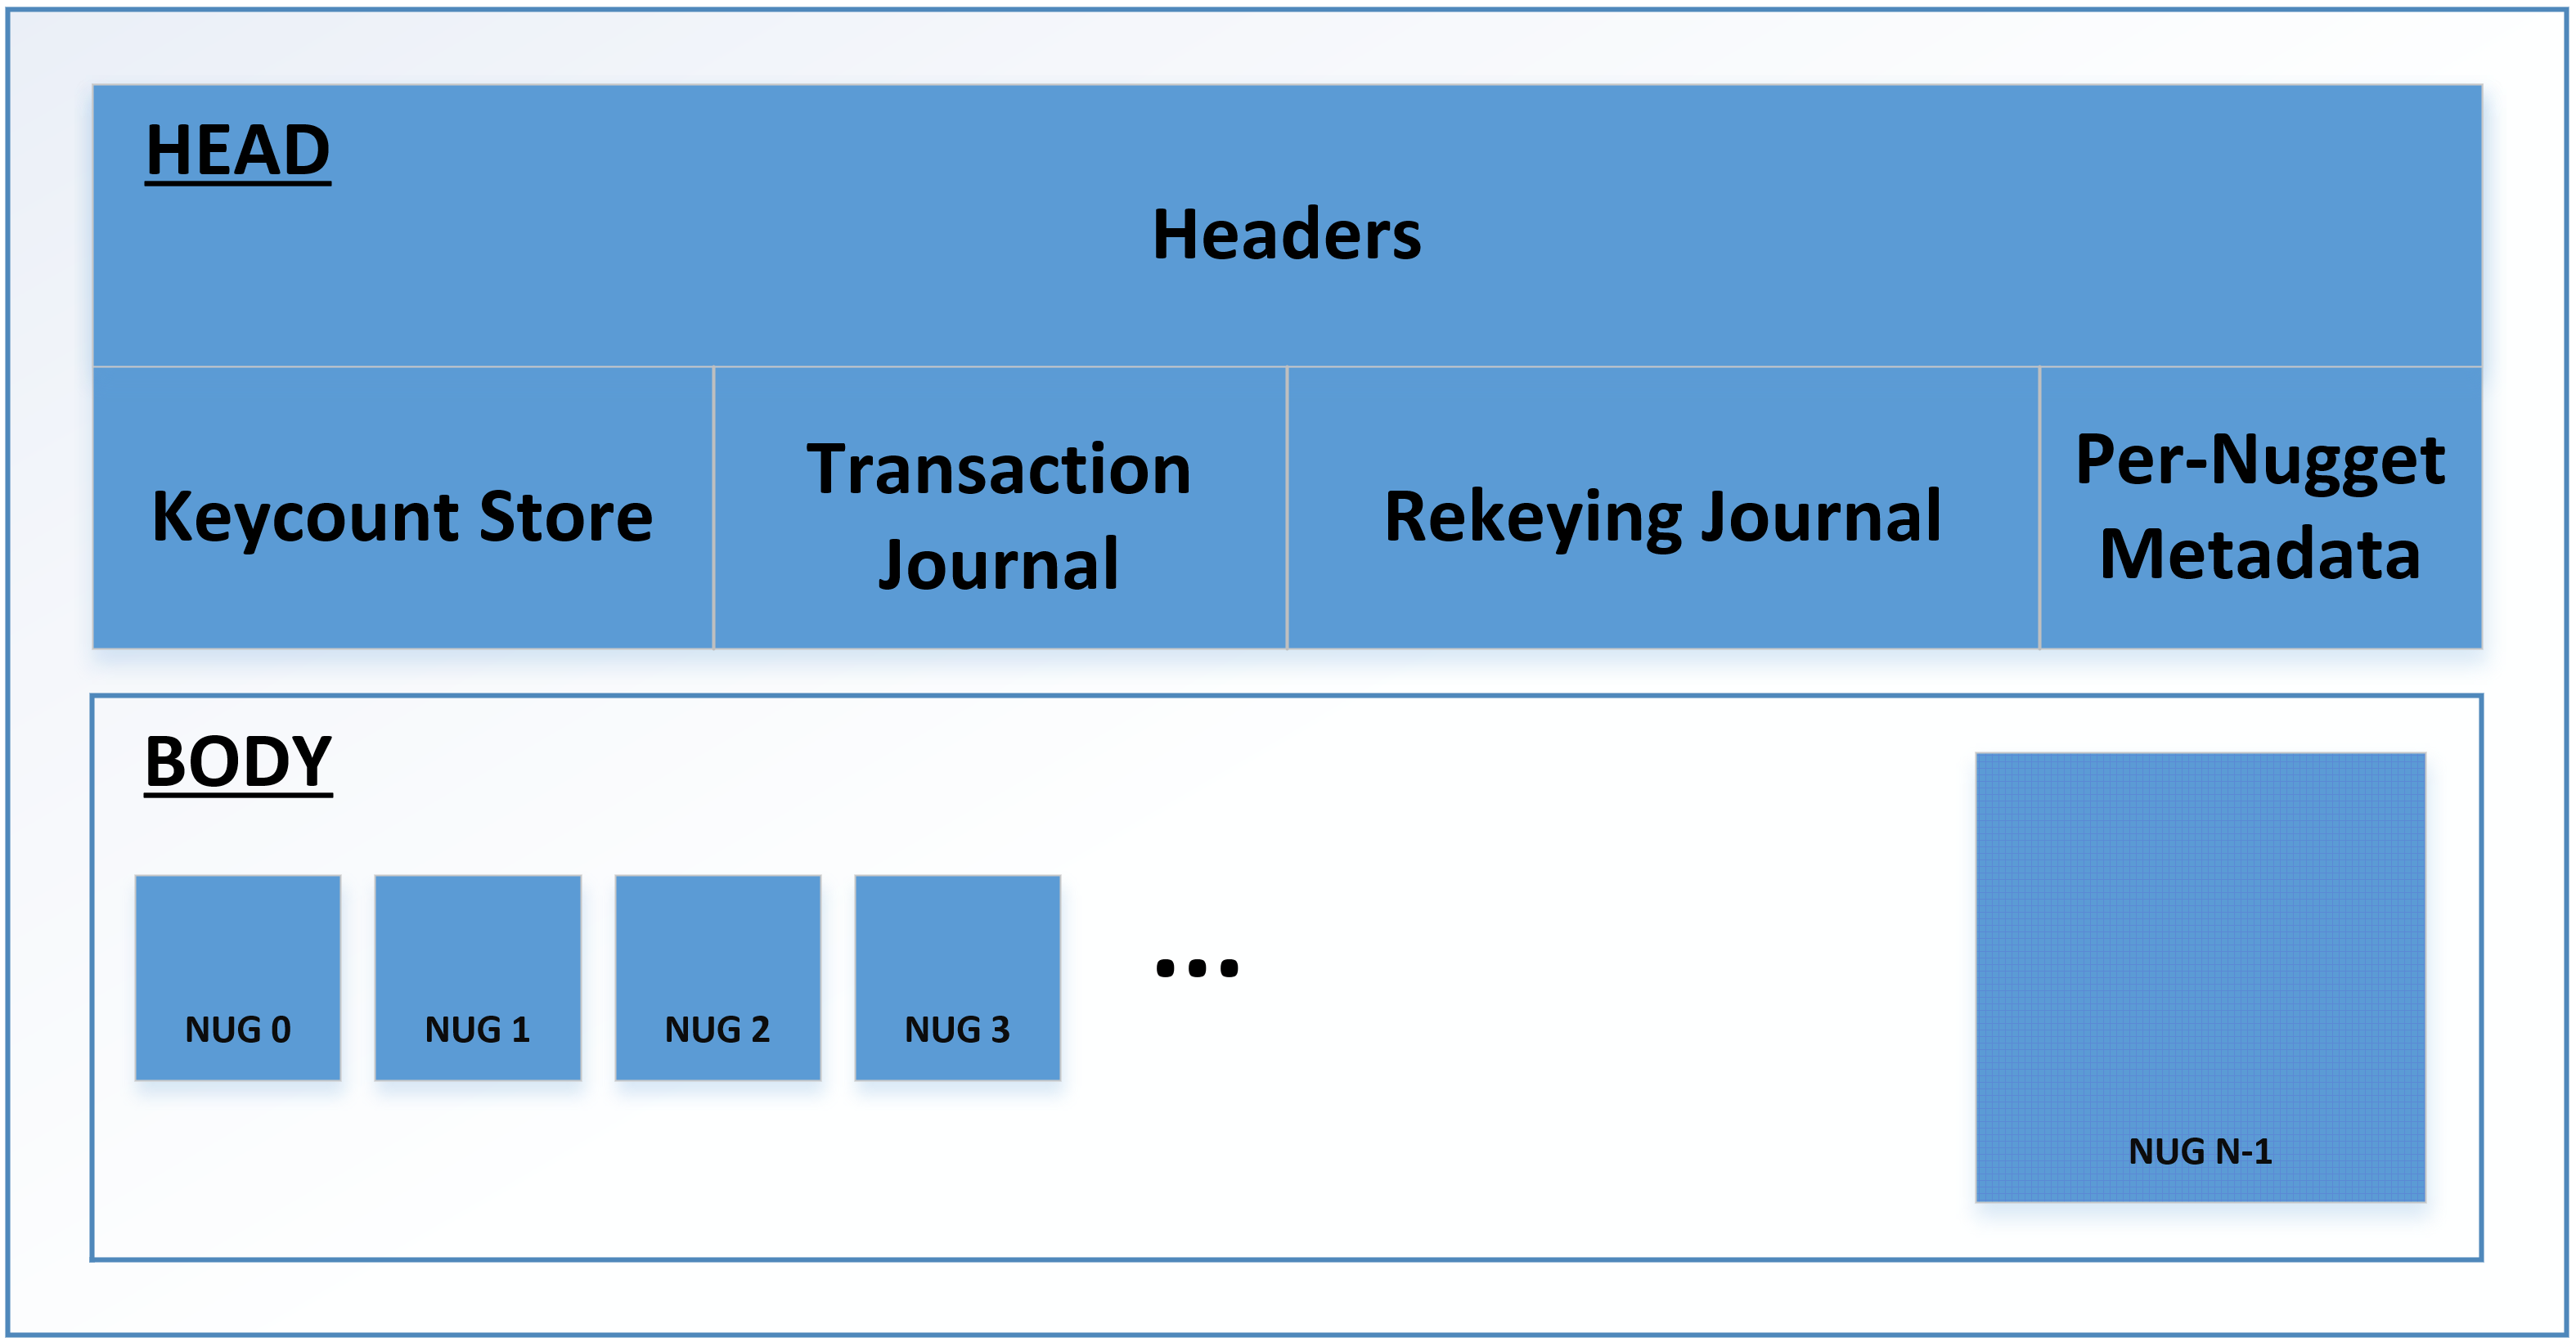
\includegraphics[width=\linewidth]{backstore.png}
   \caption{Layout of \SYSTEM{}'s backing storage.}\label{fig:backstore}
\end{figure}
